\chapter{Background}
\label{cha:background}

Insert smart intro here:

"I'm SMAAAART!!!"

\section{Rise of Dark Silicon, and the four areas of solution}
\label{sec:dark-silicon}
As Taylor\cite{dark-silicon} points out, transistor density on a CMOS chip continue to double every two years, according to Moore's Law.
Native transistor speed also increases with a factor of 1,4x.
Energy efficiency on the other hands improves only with 1,4x, and under a constant power budget, it will cause a 2x shortfall in energy budget to power a chip at its native frequency.
The utulization of a chip's potential is thus falling expentionally by 2x per generation.
If the power limitation were to be based on the current generation, then designs would be 93,75\% dark in eight years.
This gives the rise to the term "Dark Silicon", the chip must either be underclocked, or parts of it turned off in order to keep within a set power budget.
This is essentially true for chips where \todo{Hmmm.... sounds cliche} traditional cooling no longer can be efficient enough to \todo{source needed}remove generated heat from a fully powered chip.

According to Dennard scaling, progress were measured by the improvement in transistor speed and count, while according to the new post-Dennard scaling the progress will now be measured by improvement in transistor energy efficiency.
While reducing delays have been the previous focus, the focus will now be to utilize as much joule from the transistors as possible.

The transistion from single-core to multicore processors in 2005 was a direct response from the industry to this problem, but adding multiple cores does not circumvent the problem on a longer run.
Multicore chips will not scale as transistors shrink, and the fraction of a chip that can be filled with cores running at full frequency is dropping exponentially with each processor generation. 
Large fractions of the chip will be left dark - either idle for a long time, or significantly underclocked.
Hence new designs are required, where new architectural techniques "spend" area to "buy" energy efficiency.

\subsection{The Utilization Wall}
\todo{Tror dette blir overflødig, men har lagt av plass sånn i tilfelle}
Considered optional for now.
If written, should contain the details of why there is the Utulization Wall that leads to dark silicon. 

\subsection{The four horsemen: Approaches to the dark silicon problem}
Taylor explains a taxonomy called "The four horsemen" \cite{dark-silicon}.
These are four proposed responses that are emerging as solutions as one transition beyond the transitional multicore stop-gap solution. \cite{dark-silicon2}
When looking back, these responses appeared to be unlikely candidates from the beginning, bringing with them unwelcome burdens in design, manufacturing and programming.
From an aestethic engineering point of view, none of them would appear ideal.
Henceforth the term "Horsemen".
But it can be seen from the success of complex multi-regime devices like MOSFETs that engineering as a field has an enormous tolerance for complexity if the end result is better.
From this result, Taylor argues that future chips will apply not just one of these alternatives, but all of them.

The four horsemen are called The Shrinking Horseman, The Dim Horseman, The Specialized Horseman and The Dues Ex Machina Horseman.

\subsubsection{The Shrinking Horseman}
Instead of having dark silicon on the chip, one may simply shrink the chip itself.
Taylor\cite{dark-silicon} views these "shrinking chips" as the most pessimistic outcome.
Although all chips may eventually shrink somewhat, the ones that shrink the most will be those where dark silicon cannot be applied fruitfully to improve the product.
\todo{Nært overflødig?}These chips will rapidly turn into low-margin businesses for which further generations of Moore’s law provide small benefit.
Futhermore, there are other effects: Exponentially smaller chips are not exponentially cheaper, since mask cost, design cost and I/O pad aread cannot be amortized. 
Competition will most likely favor chips that utulizes dark silicon to improve overall product, causing chips that are only shrinked to sell at low market price, causing loss to the company.
And last, but not least, exponential shrinking leads to exponential rise in power density, and chip temperature will thus follow suit.
Meeting the temperature limit will reduce the scaling below the nominal 1,4x expected energy efficienty. 

%There are also second-order effects assosiated with shrinking chips:

%\begin{itemize}
%    \item Exponentially smaller chips are not exponentially cheaper.
%    In addition to the silicon itself, cost include mask costs, design costs and I/O pad area.
%    These cannot be amortized, and the price will increase per mm$^2$, as the chip shrinks.
%    \item Shrinking the silicon can also shrink the chip selling price, but competition will likely force companies to utilize dark silicon if it can attain a benefit for the end product.
%    Companies who would rely on shrinking only, may loose the competition and sell chips at catastrophically decreased chip prices.
%    \item Exponential shrinking leads to exponential rise in power density, and chip temperature will thus follow suit.
%    Meeting the temperature limit will reduce the scaling below the nominal 1,4x expected energy efficienty. 
%\end{itemize}

\subsubsection{The Dim Horseman}
%\todo{This subchapter ended up long. Try to see if it can be reduced. Especially NTV}
According to Taylor\cite{dark-silicon}, as exponentially larger fractions of a chip’s transistors become dark transistors, silicon area becomes an exponentially cheaper resource relative to power and energy consumption.
Therefore new architectural techniques that spend area to buy energy efficiency is called for.
Instead of shrinking silicon, one may consider populating dark silicon area with logic that is used only part of the time, and interesting new design possibilities occurs.
The term "dim silicon" refers to techniques that put large amounts of otherwise-dark silicon area to productive use by employing heavy underclocking or infrequent use to meet the power budget.
The architecture has to strategically managing the chip-wide transistor duty cycle to enforce the overall power constraint. 
Whereas early 90-nm designs such as Cell and Prescott were dimmed because actual power exceeded design-estimated power, more increasingly more elegant methods are converging, that make better trade-offs.
Among the dim silicon techniques are dynamically varying the frequency with the number of cores being used, scaling up the amount of cache logic, employing near threshold voltage (NTV) processor designs, and redesigning the architecture to accommodate bursts that temporarily allow the power budget to be exceeded, such as Turbo Boost and computational sprinting.

%\todo{Consider shorting down or removing entire lists from each sub-chapter, to keep the four horsemen short and concise.}Amond dim silicon methods are: 

%\begin{itemize}
%    \item Turbo boost, where less core are active, the higher the frequency they may run at.
%    Energy gained from turning off cores is used to increase voltage and frequency of active cores.
%    This is known as Dynamic voltage and frequency scaling (DVFS).
%    \item Near-threshold voltage (NTV) Processors.
%    Transistors were at 2013 operated around 2,5x the threshold voltage, an energy-delay optimal point. 
%    This is at a point where reducing the voltage severely affects the frequency drop, which reduces the effective gain from downward-DVS.
%    Nevertheless, researchers have begun exploring this regime.
%    NTV logiv is a recent approach, where transistors in the near-threshold regime are operated slightly above the threshold voltage.
%    This provides a more palatable trade-off between energy and delay than subthreshold circuits, for which frequency drops exponentially with voltage decreases.
%    \todo{Give a proper mention of where the following numbers were taken from}
%    Although NTV per-processor performance drops faster than the corresponding savings in energy-per-instruction (5X energy improvement for an 8x performance cost), the perfor- mance loss can be offset by using 8x more processors in parallel if the workload allows it.
%    Then, an additional 5x processors could turn the energy efficiency gains into additional performance. 
%    \todo{Have to admit, I still don't understand how this is a gain. And this is almost the point of too much. Should remove the example, and find a different way to explain}So, with ideal parallelization, NTV could offer 5x the throughput improvement by absorbing 40x the area. 
%    But this would also require 40x more free parallelism in the workload relative to the parallelism consumed by an equivalent energylimited super-threshold many-core processor.
%    \item Bigger caches.
%    Because only a subset of cache transistors (such as a wordline) is accessed each cycle, cache memories have low duty cycles and thus are inherently dark. 
%    Adding cache is therefore one way to simultaneously increase performance and lower power density per square millimeter.
%    But the less memory-bound a running application is, the less the benefit.
%    \item Computational sprinting and turbo boost.
%    One temporarily exceeds the nominal thermal budget but relies on thermal capacitance to buffer against temperature increases, and then ramp back to a comparatively dark state.
%    These are used within "race to finish" computations.

%\end{itemize}

\subsubsection{The Specialized Horseman}
This is the use of dark silicon to implement a host of specialized processors\cite{dark-silicon}.
They can be more energy efficient, or much faster than a general purpose processor.
Programs are executed where it is most efficient.
Unused cores are power- and clock gated in order to keep them from wasting energy.
\todo{Sort of ambigious on its own. Consider removal of sentence}
Specialized logic focuses on reducing the amount of capacitance that needs to be switched to perform a particular operation.

Specialization is already being realized today in forms of specialized accelerators that span diverse areas such as baseband processing, graphics, computer vision, and media coding.
These accelerators enable orders-of-magnitude improvements in energy efficiency and performance, especially for computations that are highly parallel.
It is expected to se a rise of systems with more coprocessors than general processors.
Tayler refers to them as coprocessor- dominated architectures, or CoDAs.

One of the expected challenges it the so-called "Tower of Babel" crisis, as the notion of general-purpose computation is fragmented, and the traditional clear lines of communication between programmers and software and the underlying hardware is eliminated.
For instance, CUDA for NVidia GPUs is not usable for similar architectures, such as AMD.
Overspecialization problems between accelerators that cause them to become inapplicable to closely related classes of computation has been observed.
In addition, adoption problems are also caused by the excessive costs of programming heterogeneous hardware (such as Sony Playstation 3 vs. Microsoft XBox), and there is always the risk that specialized hardware may become obsolete as standards are revised.

%\todo{The following sections are expanding challenges to the specialized horseman, beyond the basic. Consider carefully if this delves in too deply of our own project report, and delete it all if so.}
%The following challenges needs to be adressed:
%\begin{itemize}
%    \item To combat the "Tower of Babel" problem, it is required to define a new paradigm for how specialization is expressed and exploited in future processing systems. 
%    New scalable architectural schemas that employ pervasively specialized hardware to minimize energy and maximize performance are needed. At the same time they need to insulate the hardware designer and programmer from such systems’ underlying complexity.
%    \item  Amdahl’s law adds issues for specialization.
%    To save energy across the majority of the computation, broad-based specialization approaches that apply to both regular, parallel code and irregular code must be found.
%    It must also be ensured that communicating specialized processors doesn’t fritter away their energy savings on costly cross-chip communication or shared-memory accesses. 
%    \item Recent efforts. The UCSD GreenDroid processor. \todo{YEP!}Proposal: This is an example. Move and describe it in related works.
%\end{itemize}

\subsubsection{The Dues Ex Machina Horseman}
Taylor notes that this one is the most unpredictable\cite{dark-silicon}.
He uses the termology "Deus ex machina" from literature or theater, in which the protagonists seem increasingly doomed until the very last moment, when something completely unexpected comes out of nowhere to save the day.
In the case for dark silicon, one deus ex machina would be a breakthrough in semiconductor devices.
The required breakthrough would have to be very fundamental, making it possible to build transistors out of devices other than MOSFETs. 
There are physical limits to what can be done with \todo{I chose to not elaborate this one further}leakage from MOFSET transistors, and transistors made of other devices can combat this.
New transistors must also be able to compete with MOFSETs in performance.
Tunnel field-effect transistors (TFET) and nanoelectromechanical system (NEMS) switches are examples on inventions that hint to order-in-magnitude improvements in the leakage problem, but they still fall short in performance.

% TODO: Remove all occurrences of the word "horseman", it's a litterary reference we shouldn't use.

\section{Heterogeneous Architectures}
\label{sec:heterogeneous}


\subsection{The Single-ISA Heterogeneous MAny-core Computer}
\label{sec:shmac}
The Single-ISA Heterogeneous MAny-core Computer is a proposed infrastructure by NTNU for investigating heterogeneous systems at all abstraction levels, as illustrated in figure \cite{fig:shmacAbstractionLevels}.
The point is to create a flexible framework in which different heterogeneous processors can be created from a collection of processing elements and accelerators.
The programming model is kept constant across SHMAC-instances, while underlying implementation changes.
This way, software design space exploration is facilitated.
It is a tile-based architecture with a mesh interconnect.
All processor tiles implement the same ARM ISA and the same memory model, in order to achieve a common programming model.\cite{shmac-plan}.
An illustration of SHMAC can be seen in figure \cite{fig:shmac}.

\begin{figure}[htb]
    \centering
    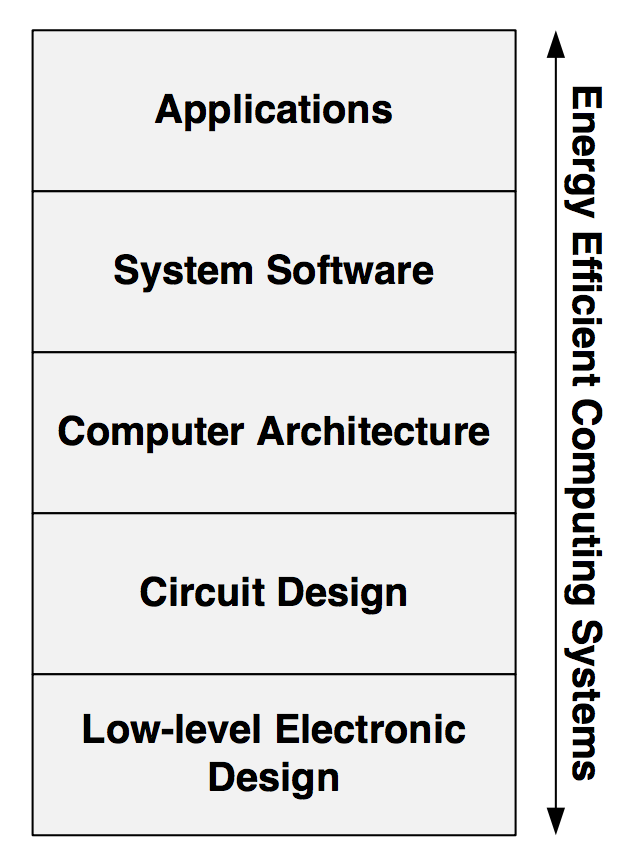
\includegraphics[width=0.5\textwidth]{Figures/Heterogeneous/SHMACAbstractionLevels}
    \caption{All levels of abstraction in computing systems, as seen in \cite{shmac-plan}.}
    \label{fig:shmacAbstracionLevels}
\end{figure}

\begin{figure}[htb]
    \centering
    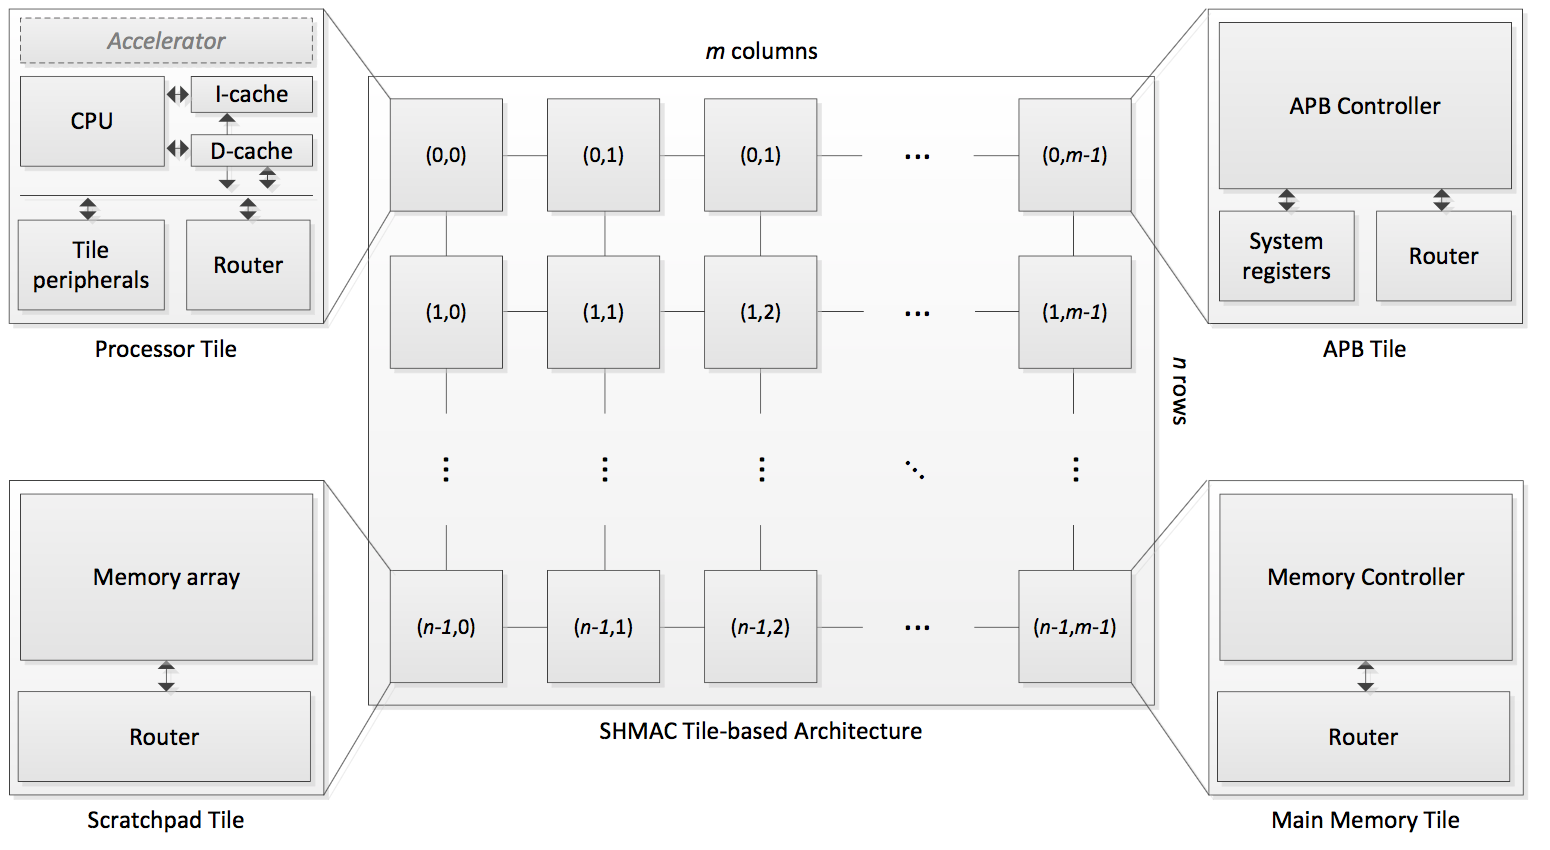
\includegraphics[width=1.0\textwidth]{Figures/Heterogeneous/SHMAC}
    \caption{High-Level Architecture of ARM-based SHMAC, as seen in \cite{shmac-plan}.}
    \label{fig:shmac}
\end{figure}

\todo{PROBLEM: This paragraph is way too similar to original text. Must fix, one way or another. }NTNU argues that the SHMAC-approach gives the right tools to reach the research goles outlined in the plan in \cite{shmac-plan}.
For software research, SHMAC, makes it possible to explore substantially more diverse systems than the ones currently provided by the industry.
Furthermore, SHMAC-architectures realized in FPGAs will be significatly faster than using simulators.
It is expected that co-developing software and hardware will result in substantial cross-fertilization that gives insight into both hardware and software issues.
And finally, micro- and macro-architecture components can be combined with novel transistor technologies and ASIC realizations to reach research goals at the lower abstraction levels.

%Original source, kept for source comparison
%We believe that the SHMAC-approach gives us the right tools to reach the research goals outlined in this plan. For software research, SHMAC makes it possible to explore substantially more diverse systems than those cur- rently provided by the industry. At the same time, SHMAC-architectures realized in FPGAs will be significantly faster than simulator-based approaches. We expect that co-developing software and hardware result in substan- tial cross-fertilization that gives insights into both hardware and software issues. Finally, the SHMAC micro- and macro-architecture components can be combined with novel transistor technologies and ASIC realizations to reach research goals at the lower abstraction levels.

\subsubsection{SHMAC Architecture}

\subsubsection{Work packages}


\section{The Bitcoin Currency}
\label{sec:bitcoins}

Bitcoin is a new currency, based on cryptographic stuffz\todo{Eloquence}.

At the core of the bitcoin system is the block chain, a distributed linked-list consisting of blocks
which contains the transactions that have been executed since the previous block was generated.

A block is only valid if the arithmetic value of the double SHA-256 hash of its header is below
a certain target value. The target value is decided by the network and is set to such a value that
on average six new blocks are generated per hour. \cite{bitcoin}

\subsection{Mining Bitcoins}
\label{sec:bitcoin-mining}

The process of creating a new block for the bitcoin blockchain is often referred to as \textit{mining}.

The process begins with the creation of a transaction that transfers the reward for generating the block
into the account of the miner. This transaction is called the coinbase transaction. All transactions
transmitted to the bitcoin network since the last block was generated are gathered and a merkle tree
is constructed by combining the hashes of these transactions\todo{Explain merkle trees}.

The root of the merkle tree is inserted into the header for the new block together with the hash of the
previous block and various other fields specified by the standard. If the hash is below a target value,
determined by the current network difficulty, the block is successfully mined and transmitted to the
network.
